\chapter{Cơ sở lý thuyết}
\label{chap:theory}

% =====================================================================
\section{Tổng quan YOLO và phân đoạn thực thể với YOLO11-seg}
\label{sec:yolo}

\emph{Phát hiện đối tượng} (object detection) xác định vị trí (hình chữ nhật bao) và nhãn lớp của từng đối tượng trong ảnh.
\emph{Phân đoạn thực thể} (instance segmentation) đi xa hơn: với mỗi đối tượng, mô hình trả về một mặt nạ nhị phân
$M \in \{0, 1\}^{H \times W}$, tức một bảng có $H$ hàng và $W$ cột tương ứng với chiều cao và chiều rộng ảnh: giá trị 1 đánh dấu điểm ảnh thuộc đối tượng, giá trị 0 là không thuộc đối tượng đó. Mỗi xe có mặt nạ riêng nên hai xe cùng lớp đứng cạnh nhau vẫn được phân biệt.

YOLO (You Only Look Once)~\cite{redmon2016yolo} xử lý toàn ảnh để dự đoán trực tiếp vị trí và lớp của các đối tượng:
mạng dùng các bộ lọc để trích thông tin từ ảnh, rồi dự đoán đồng thời toạ độ hộp, độ tin cậy và điểm của từng lớp, nên phù hợp với yêu cầu xử lý nhanh; tốc độ thực tế còn phụ thuộc ảnh đầu vào, mô hình và phần cứng.
YOLO11~\cite{yolo11} là phiên bản do Ultralytics phát hành năm 2024, hỗ trợ nhiều tác vụ; đồ án sử dụng phiên bản phân đoạn thực thể YOLO11-seg.

\subsection{Kiến trúc YOLO11-seg}

Kiến trúc gồm ba phần~\cite{khanam2024yolov11}, xử lý nối tiếp nhau:
\begin{itemize}
  \setlength{\itemsep}{0.35em}
  \item \textbf{Backbone} (phần trích đặc trưng): thu nhỏ ảnh dần qua nhiều tầng. Tầng nông giữ chi tiết như cạnh, góc; tầng sâu nhìn được vùng rộng hơn và nhận ra đối tượng.
  \item \textbf{Neck} (phần trộn đặc trưng): kết hợp thông tin giữa các tầng, để phát hiện được cả xe nhỏ ở xa lẫn xe lớn ở gần.
  \item \textbf{Head} (phần dự đoán): từ đặc trưng đã trộn, đưa ra hộp bao, lớp xe và thông tin để dựng mặt nạ.
\end{itemize}

Hình~\ref{fig:yolo11-arch} mô tả kiến trúc ở mức khối, trong đó P3, P4, P5 là ba mức đặc trưng từ chi tiết đến khái quát.

\begin{figure}[H]
\centering
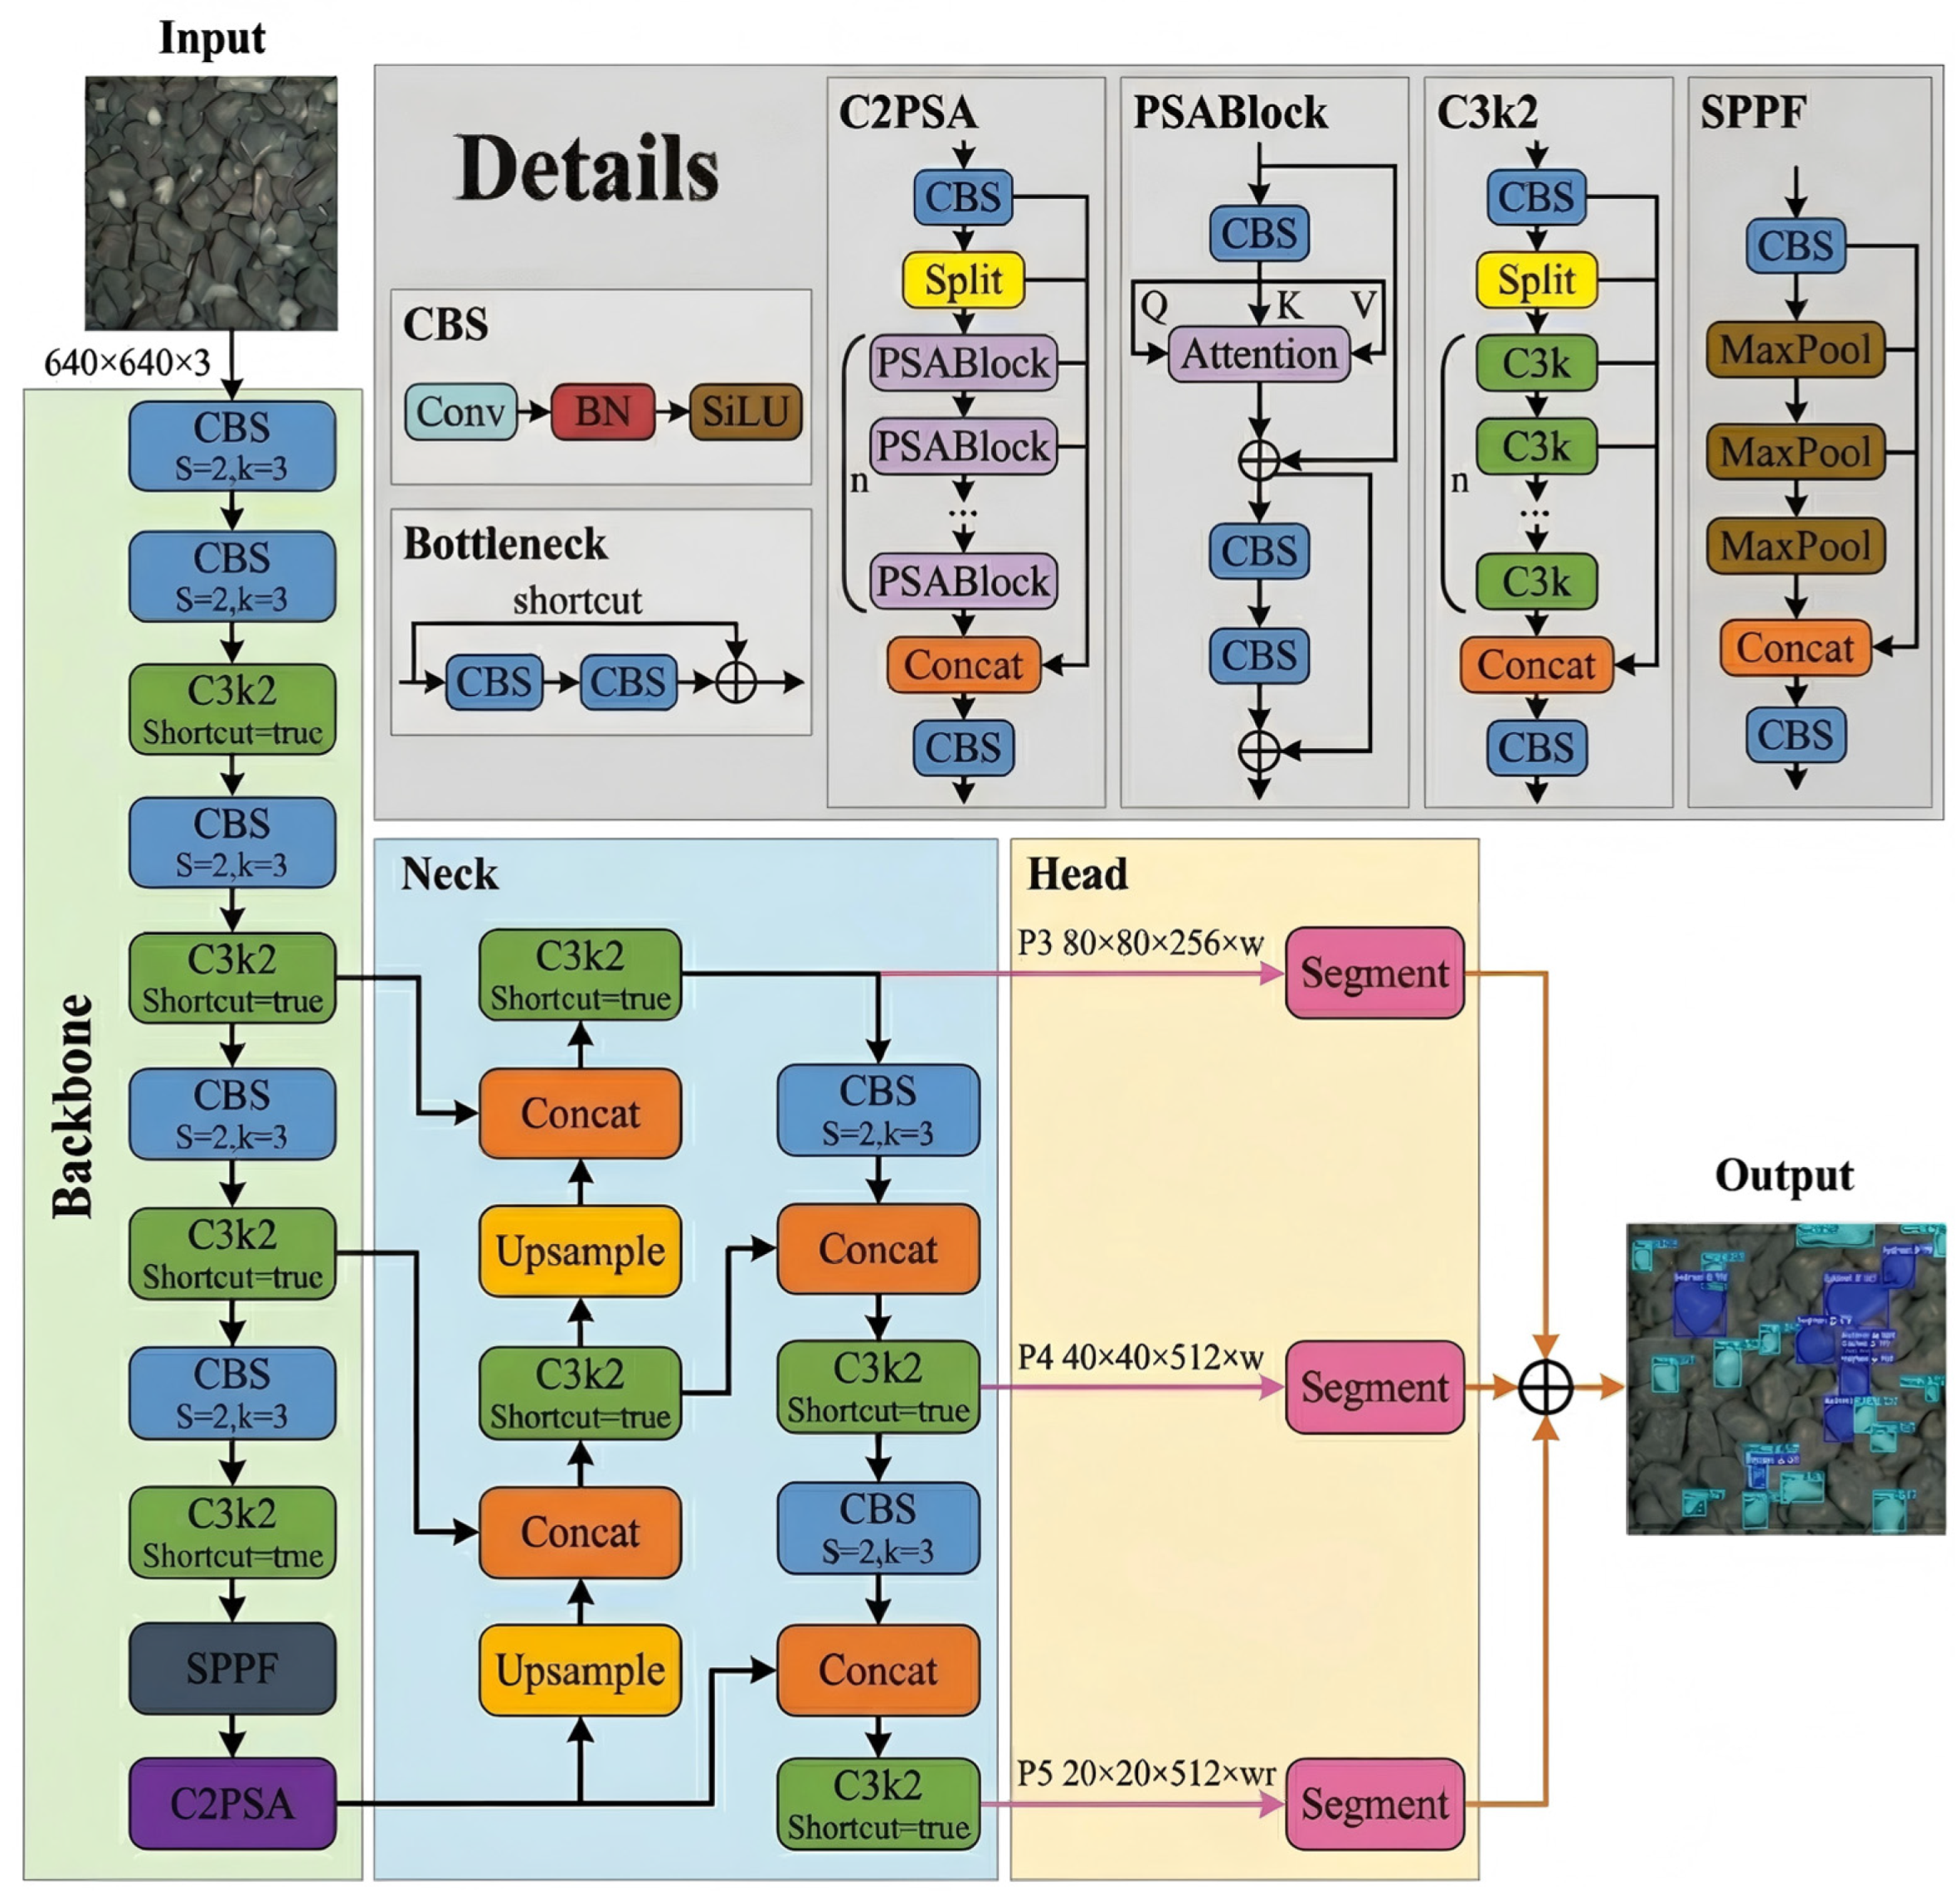
\includegraphics[width=\linewidth]{yolo11_seg_architecture.png}
\caption[Kiến trúc YOLO11-seg]{Kiến trúc YOLO11-seg, trích từ Hình~1 trong~\cite{wang2026lggyoloseg}. Kích thước ảnh đầu vào minh hoạ là $640 \times 640$.}
\label{fig:yolo11-arch}
\end{figure}

Trong hình, CBS gồm ba bước: Conv dùng bộ lọc để trích đặc trưng; BN điều chỉnh thang giá trị của các đặc trưng; SiLU biến đổi các giá trị qua hàm kích hoạt để mạng học được các quan hệ phức tạp. CBS tương ứng với khối Conv trong Bảng~\ref{tab:yolo_blocks}. Các ảnh đầu vào và đầu ra là ví dụ phân đoạn quặng của tài liệu nguồn. Bảng~\ref{tab:yolo_blocks} giải thích vai trò các khối chính của YOLO11-seg, theo tài liệu của Ultralytics~\cite{ultralytics_arch} và mã nguồn~\cite{yolo11}.

\begin{table}[H]
\centering
\caption{Vai trò của các khối trong YOLO11-seg}
\label{tab:yolo_blocks}
\begin{tabular}{>{\raggedright\arraybackslash}p{3.2cm} >{\raggedright\arraybackslash}p{11.8cm}}
\toprule
\textbf{Khối} & \textbf{Vai trò} \\
\midrule
Conv & Đơn vị cơ bản, lọc ảnh để lấy đặc trưng. Khi đặt bước nhảy 2, khối này giảm một nửa chiều cao và chiều rộng. \\
C3k2 & Khối lặp chính: cho một phần dữ liệu đi qua nhiều lớp xử lý, phần còn lại giữ nguyên rồi ghép lại, nhờ đó học được nhiều mà tốn ít phép tính. \\
SPPF & Gom thông tin từ các vùng rộng dần quanh mỗi vị trí, để mô hình nắm được ngữ cảnh xung quanh. \\
C2PSA & Dùng cơ chế chú ý (attention) để mỗi vị trí có thể tham khảo toàn ảnh và tập trung vào vùng có đối tượng. \\
Upsample, Concat & Phóng to bản đồ đặc trưng rồi ghép với bản đồ cùng kích thước. Neck dùng cách này theo hai chiều: đưa thông tin nhận dạng từ tầng sâu xuống và đưa thông tin vị trí từ tầng nông lên. \\
Segment & Tại mỗi vị trí trên ba mức đặc trưng, dự đoán hộp bao, điểm của từng lớp và 32 hệ số để dựng mặt nạ. \\
Proto & Sinh 32 \emph{mặt nạ nguyên mẫu}, là các mẫu trung gian dùng chung để tạo mặt nạ riêng cho từng đối tượng, không phải các lớp xe. \\
\bottomrule
\end{tabular}
\end{table}

Sau khi mô hình dự đoán, Non-Maximum Suppression (NMS) loại bỏ các dự đoán trùng nhau trên cùng một xe.
Mỗi xe còn lại có 32 hệ số riêng, cho biết mức đóng góp của từng mặt nạ nguyên mẫu. Mặt nạ của xe được tạo bằng cách cộng các nguyên mẫu theo những hệ số này, rồi cắt theo hộp bao, phóng về kích thước ảnh gốc và giữ các điểm ảnh có giá trị từ 0,5 trở lên.

Đồ án so sánh sơ bộ hai mô hình huấn luyện sẵn là YOLO11n-seg (nano) và YOLO11l-seg (large), rồi chọn một mô hình cho các thí nghiệm (mục~\ref{sec:model_select}). Hai mô hình có cùng sơ đồ khối ở Hình~\ref{fig:yolo11-arch}, chỉ khác về độ lớn~\cite{yolo11}.
Bản large có số tham số gấp gần 10 lần bản nano, nên nhận dạng tốt hơn nhưng chạy chậm hơn.

COCO (Common Objects in Context)~\cite{lin2014coco} là bộ dữ liệu ảnh công khai gồm 80 lớp đối tượng thường gặp, được dùng rộng rãi để huấn luyện và so sánh các mô hình. Bộ này chứa sẵn các lớp \texttt{car}, \texttt{truck}, \texttt{bus}, \texttt{motorcycle}, nên đồ án có thể dùng mô hình huấn luyện sẵn và chỉ giữ bốn lớp này khi inference (chạy mô hình để dự đoán).

Thư viện Ultralytics cung cấp tập điểm biên của từng mặt nạ qua thuộc tính \texttt{masks.xy}; đồ án sử dụng tập điểm này làm đầu vào cho thuật toán dựng bao lồi trực giao.

% =====================================================================
\section{Bao lồi trực giao}
\label{sec:och}

\subsection{Các khái niệm}

\begin{dinhnghia}[Tập lồi]
Tập $K$ trong mặt phẳng được gọi là \emph{lồi} nếu với hai điểm bất kỳ thuộc $K$, toàn bộ đoạn thẳng nối chúng cũng thuộc $K$.
\end{dinhnghia}
Nói đơn giản, khi nối hai điểm trong tập bằng một đoạn thẳng, đoạn nối không đi ra ngoài tập.

\begin{dinhnghia}[Bao lồi]
\emph{Bao lồi} của tập điểm $P$, ký hiệu $\operatorname{conv}(P)$, là tập lồi nhỏ nhất chứa $P$.
\end{dinhnghia}
Có thể hình dung căng một sợi dây thun quanh các điểm rồi thả ra: dây ôm sát các điểm ngoài cùng, còn dây và phần bên trong tạo thành bao lồi.

Trước khi định nghĩa bao lồi trực giao, một tập được gọi là \emph{lồi trực giao} nếu giao của nó với mỗi đường thẳng ngang hoặc dọc là tập rỗng, một điểm, hoặc một đoạn thẳng. Nói đơn giản, mỗi đường ngang hoặc dọc chỉ cắt tập thành nhiều nhất một đoạn liền, không thành hai đoạn rời nhau.

\begin{dinhnghia}[Bao lồi trực giao liên thông~\cite{an2021ograham,nguyen2022quickhull}]
Một bao lồi trực giao liên thông của tập điểm $P$ là một tập chứa tất cả các điểm của $P$, liền một khối, thoả mãn điều kiện lồi trực giao và không thể bỏ bớt phần nào mà vẫn giữ các tính chất này.
\end{dinhnghia}
Trong báo cáo, ``bao lồi trực giao liên thông'' được gọi tắt là ``bao lồi trực giao''.

\subsection{Cấu trúc bậc thang và đặc trưng hình học}
\label{sec:staircase}

Để hình dung cách dựng bao, trước hết xét các điểm nằm ở phía ngoài của tập điểm $P$. Từ một điểm $p$, kẻ một đường ngang và một đường dọc để chia mặt phẳng thành bốn góc phần tư: trên phải, trên trái, dưới trái và dưới phải, có tính cả các điểm nằm trên đường ngang hoặc dọc giới hạn góc đó. Nếu có ít nhất một góc phần tư không chứa điểm nào khác của $P$, thì $p$ được gọi là \emph{điểm tối đại}~\cite{nguyen2022quickhull}. Chẳng hạn, một điểm có góc phần tư trên trái trống là điểm tối đại theo hướng Tây Bắc.

Từ tập điểm $P$, tìm vị trí trái nhất, phải nhất, thấp nhất và cao nhất. Kẻ hai đường dọc và hai đường ngang qua các vị trí này, ta được \emph{hình chữ nhật bao}. Đây là khung phụ để xác định các điểm mốc, chưa phải bao lồi trực giao.

Trên cạnh trên và cạnh dưới, lấy điểm trái nhất và phải nhất; trên cạnh trái và cạnh phải, lấy điểm cao nhất và thấp nhất. Như vậy có tối đa tám \emph{điểm mốc}. Nếu một cạnh chỉ có một điểm thì hai mốc trên cạnh đó trùng nhau; điểm nằm ở góc hình chữ nhật cũng có thể là mốc của hai cạnh.

Biên của bao được chia thành bốn phần ở bốn góc, mỗi phần có dạng bậc thang (Hình~\ref{fig:four_chains}):
\begin{itemize}
  \item \textbf{Góc trên trái (Tây Bắc):} nối điểm trái nhất trên cạnh trên với điểm cao nhất trên cạnh trái.
  \item \textbf{Góc dưới trái (Tây Nam):} nối điểm thấp nhất trên cạnh trái với điểm trái nhất trên cạnh dưới.
  \item \textbf{Góc dưới phải (Đông Nam):} nối điểm phải nhất trên cạnh dưới với điểm thấp nhất trên cạnh phải.
  \item \textbf{Góc trên phải (Đông Bắc):} nối điểm cao nhất trên cạnh phải với điểm phải nhất trên cạnh trên.
\end{itemize}
Mỗi phần được gọi là một \emph{chuỗi bậc thang}. Bốn chuỗi, ghép với các đoạn nối trên bốn cạnh hình chữ nhật, tạo thành đường viền của bao.

\begin{figure}[H]
\centering
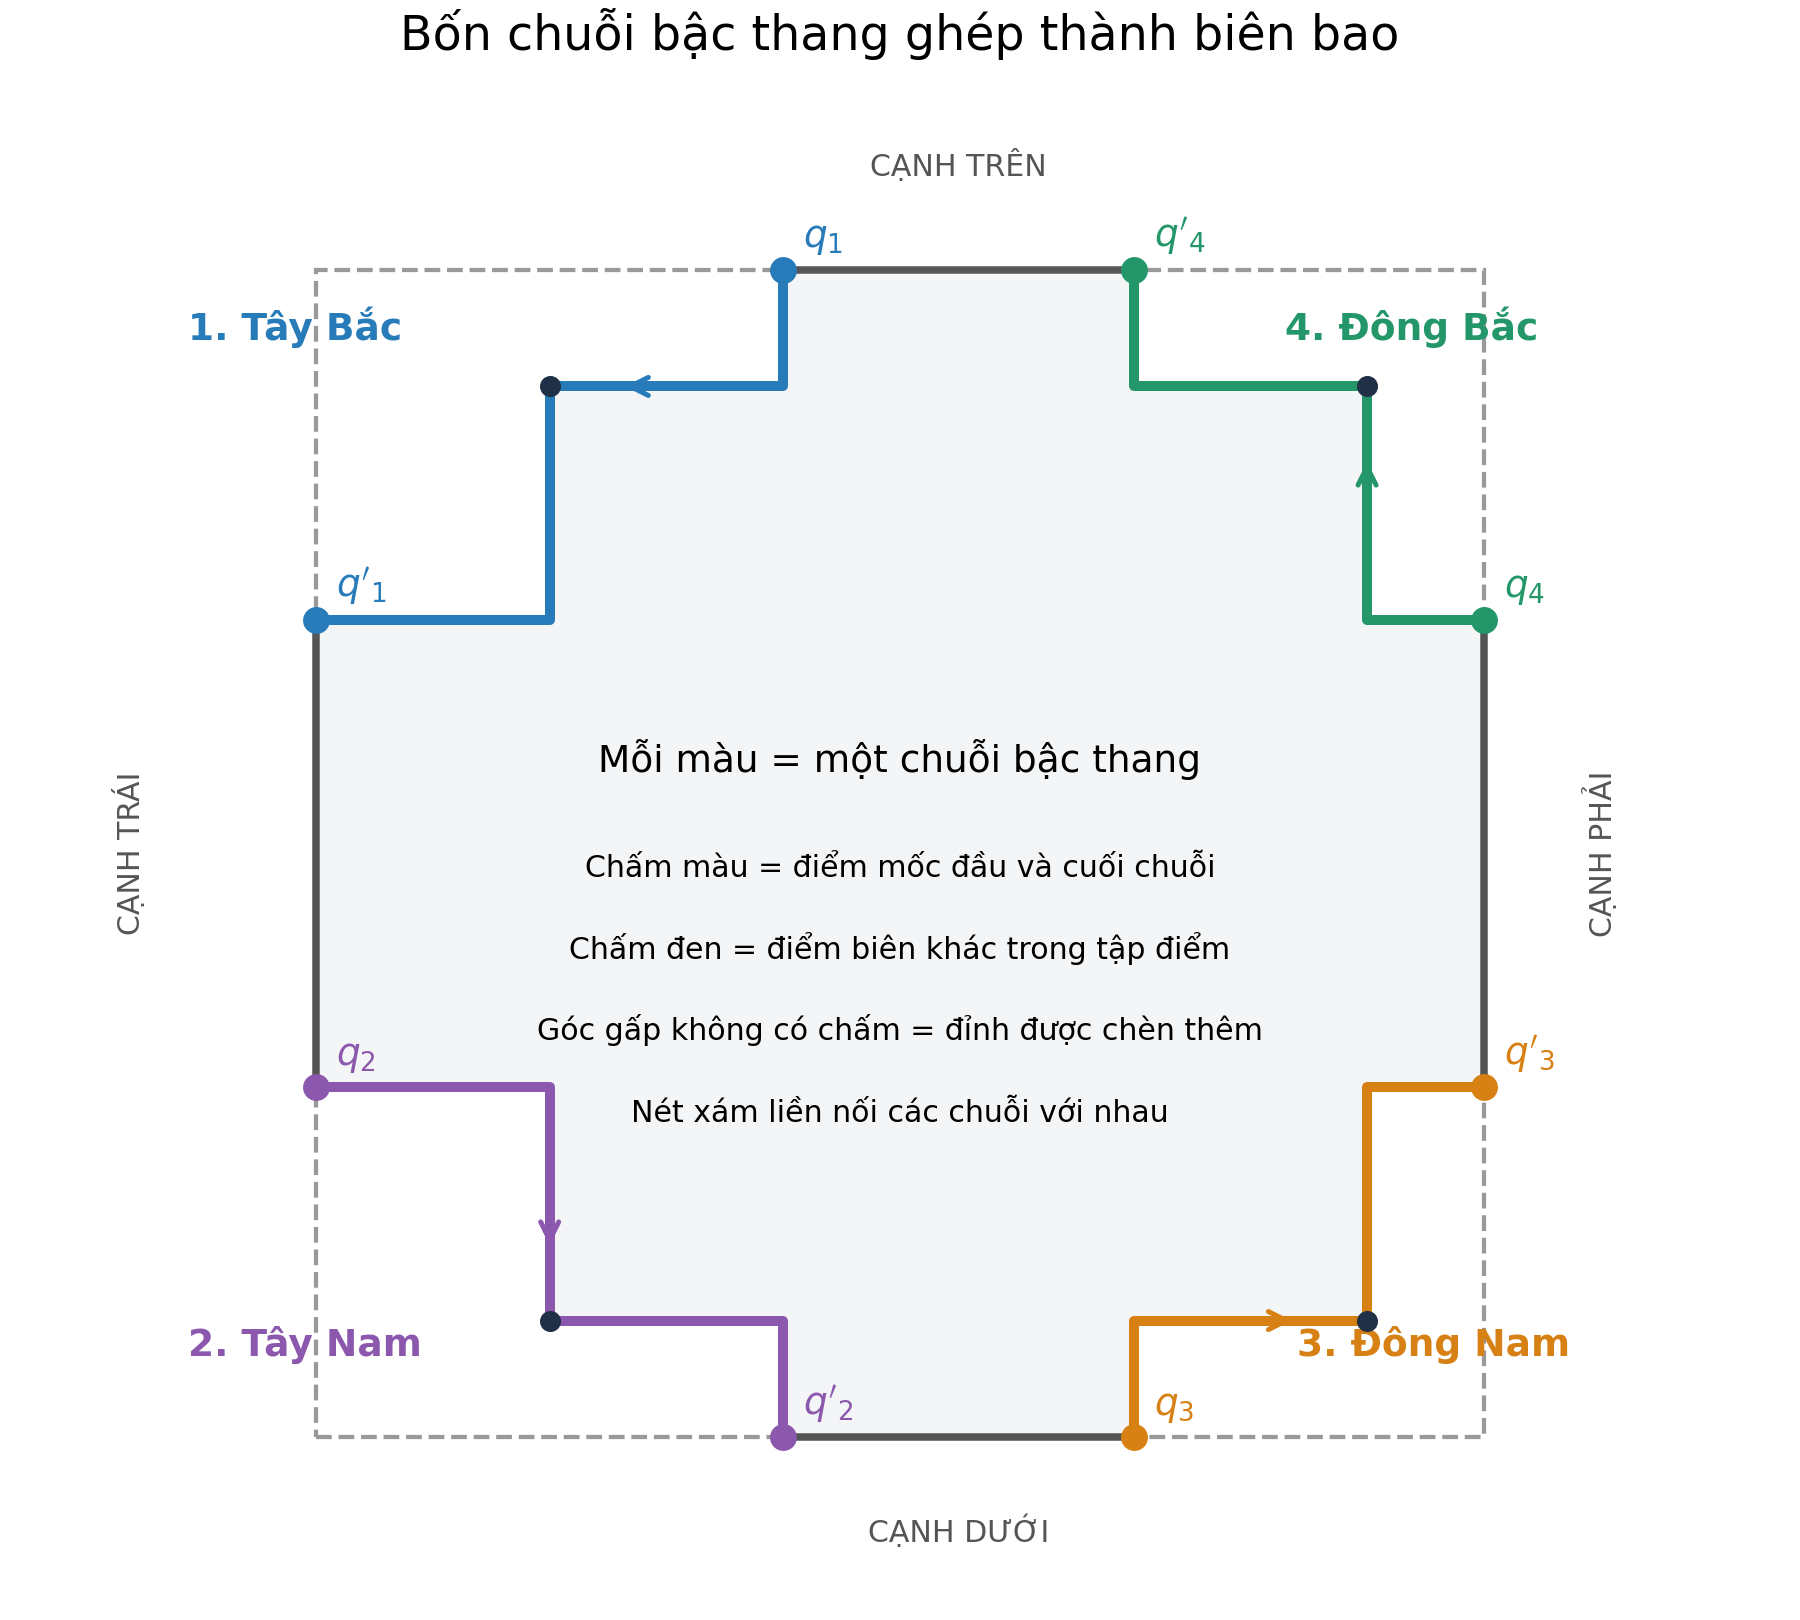
\includegraphics[width=0.92\linewidth]{four_staircase_chains.png}
\caption{Minh hoạ bốn chuỗi bậc thang bằng bốn màu. Các chấm màu là điểm mốc đầu và cuối chuỗi; các đoạn xám liền nối các chuỗi. Khung nét đứt là hình chữ nhật bao.}
\label{fig:four_chains}
\end{figure}

Các điểm của $P$ được chọn trên mỗi chuỗi là điểm tối đại theo hướng tương ứng~\cite{nguyen2022quickhull}. Khi hai điểm liên tiếp nằm chéo nhau, ta nối chúng bằng một đoạn ngang và một đoạn dọc. Chỗ rẽ là một góc vuông được chèn thêm về phía trong bao, không nhất thiết thuộc $P$. Trong Hình~\ref{fig:four_chains}, các góc gấp không có chấm chính là những đỉnh được chèn thêm. Hình~\ref{fig:hull_illus} minh hoạ kết quả trên một tập 28 điểm.

\begin{figure}[H]
\centering
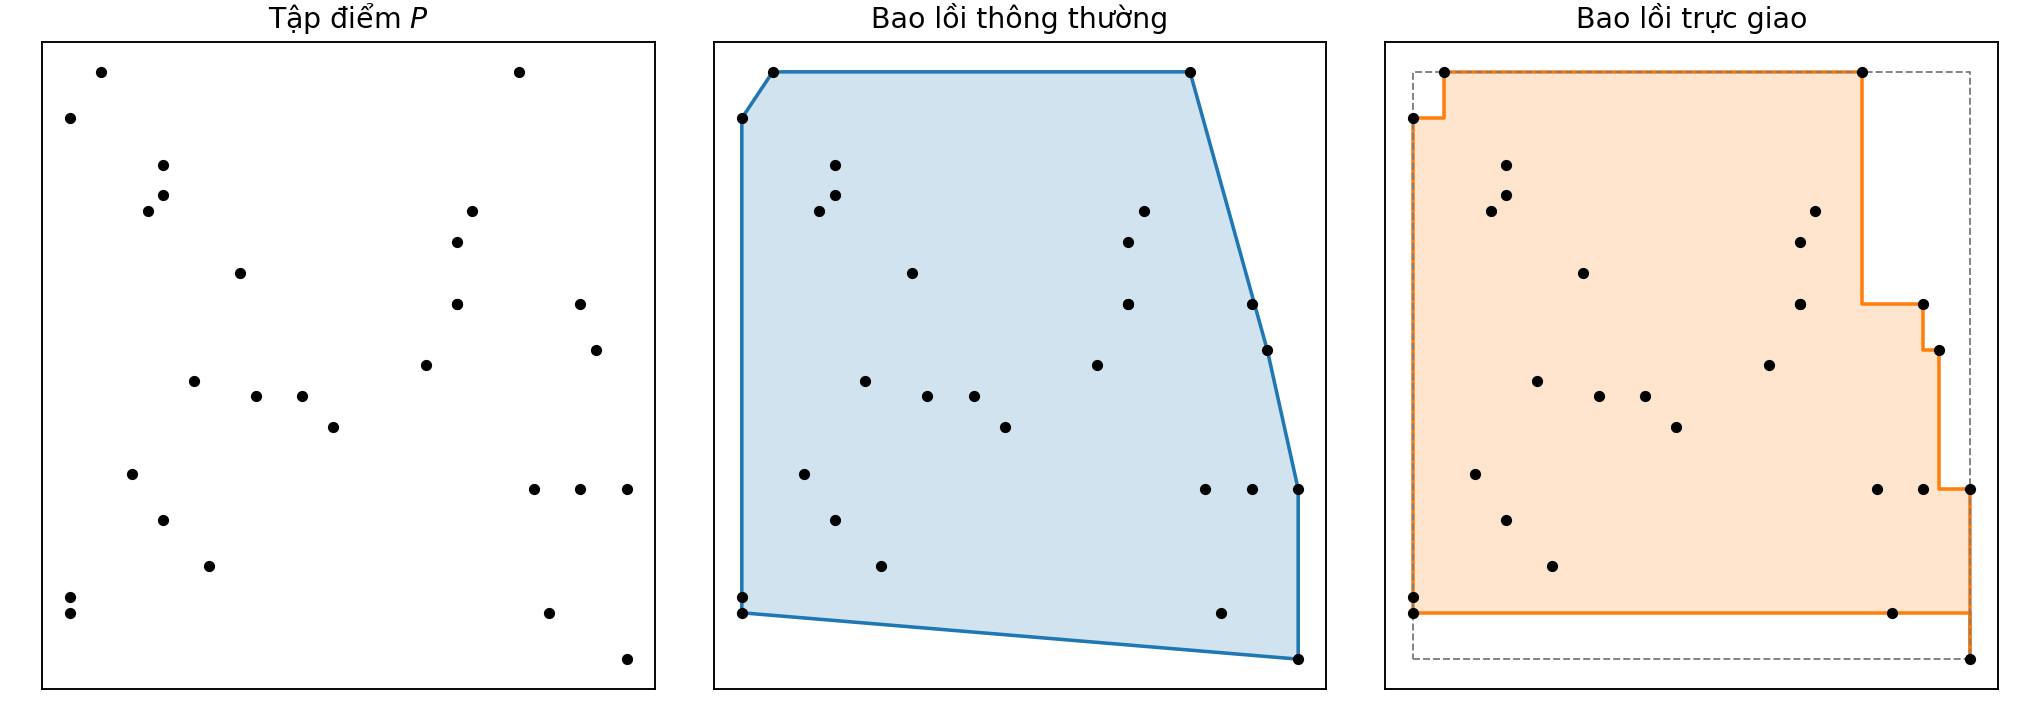
\includegraphics[width=0.98\linewidth]{hull_illustration.png}
\caption{Một tập điểm (trái), bao lồi thông thường (giữa) và bao lồi trực giao liên thông (phải); nét đứt là hình
chữ nhật bao. Đoạn thẳng đứng ở góc dưới phải nối điểm thấp nhất vào phần còn lại của bao; đa giác trực giao trong~\cite{nguyen2022quickhull} cho phép có các đoạn thẳng như vậy.}
\label{fig:hull_illus}
\end{figure}

\begin{nhanxet}
\label{rem:inclusion}
Bao lồi trực giao liên thông và bao lồi thông thường đều chứa $P$ và đều nằm trong hình chữ nhật bao.
Tuy nhiên, bao trực giao liên thông không phải lúc nào cũng nằm trong bao lồi thông thường:
khi các điểm thẳng hàng theo đường chéo, bao lồi chỉ là một đoạn thẳng, còn đường nối trực giao phải đi ra ngoài đoạn đó.
Vì vậy, mức nền thừa và khả năng biểu diễn hình dạng của các loại bao
cần được so sánh bằng thực nghiệm trên dữ liệu cụ thể; kết quả của đồ án được trình bày ở Chương~\ref{chap:exp}.
\end{nhanxet}

Diện tích của đa giác bao được tính từ toạ độ các đỉnh, còn chu vi là tổng độ dài các cạnh.
Trong đầu ra video, tỉ lệ lấp đầy được tính bằng diện tích bao chia cho diện tích hộp phát hiện YOLO, cho biết vùng bao chiếm bao nhiêu phần của hộp. Hộp YOLO được mô hình dự đoán riêng, nên có thể khác hình chữ nhật tính từ các điểm biên. Các đối tượng có dựng bao được lưu những đặc trưng này vào tệp CSV (bảng dữ liệu dạng văn bản).

% =====================================================================
\paragraph{Tính duy nhất của bao.}
Một tập điểm có thể có nhiều bao lồi trực giao liên thông hợp lệ~\cite{an2021ograham,nguyen2022quickhull}. Hai bản cài đặt dùng quy tắc nối cố định để tạo đầu ra. Quy tắc nối cố định không tự bảo đảm bao tối tiểu và duy nhất trên mọi tập điểm.

\section{Bản QuickHull của nhóm}
\label{sec:quickhull}

QuickHull là ý tưởng tìm biên bằng cách chọn điểm rồi tiếp tục xử lý các tập điểm nhỏ hơn~\cite{eddy1977,barber1996}. O-Quickhull áp dụng ý tưởng chia để trị cho bao lồi trực giao~\cite{nguyen2022quickhull}. Đồ án dùng một bản QuickHull chọn điểm theo toạ độ, không tái hiện bước chọn điểm xa góc gấp nhất và chia hai nhánh của O-Quickhull gốc. Các bước, giả mã và hình trong mục này mô tả bản cài đặt thực tế của nhóm. Trong báo cáo, hai bản cài đặt được gọi ngắn là \emph{bản QuickHull} (bản đệ quy chọn điểm theo toạ độ) và \emph{bản Graham} (bản sắp xếp--quét theo ý tưởng O-Graham); các tên ngắn này không khẳng định nhóm tái hiện nguyên thuật toán gốc.

Trong bản QuickHull này, việc chọn điểm theo toạ độ có nghĩa là chọn điểm có toạ độ cao nhất, thấp nhất, trái nhất hoặc phải nhất theo hướng đang xét. Đây là cách chọn theo toạ độ, không phải khẳng định mọi điểm được chọn đều là điểm cực trị của bao trên mọi đầu vào.

Trước hết, tìm tối đa tám điểm mốc và chia tập điểm thành bốn vùng ứng với bốn chuỗi bậc thang ở mục~\ref{sec:staircase}. Gọi hai mốc đầu--cuối của chuỗi thứ $k$ là $(q_k,q'_k)$, với $k=1,2,3,4$ lần lượt ứng với Tây Bắc, Tây Nam, Đông Nam và Đông Bắc.

Với chuỗi Tây Bắc, bản cài đặt xử lý như sau:
\begin{enumerate}
  \item \textbf{Lấy tập điểm cần xét.} Giữ các điểm trong hình chữ nhật có hai đỉnh đối diện là hai mốc của chuỗi, bỏ chính hai mốc. Gọi tập này là $S$; nếu $S$ rỗng thì không cần tìm thêm điểm trung gian.
  \item \textbf{Chọn hai điểm theo toạ độ.} Chọn điểm cao nhất của $S$; nếu có nhiều điểm cùng độ cao thì lấy điểm bên trái nhất. Tiếp đó, chọn điểm trái nhất của $S$; nếu có nhiều điểm cùng vị trí ngang thì lấy điểm cao nhất. Mã thực hiện việc này bằng hai lần sắp xếp.
  \item \textbf{Thu hẹp tập cần xử lý.} Giữ các điểm trong hình chữ nhật giữa hai điểm vừa chọn, bỏ chính hai điểm đó. Áp dụng lại bước chọn điểm cho tập nhỏ hơn này. Mỗi lần chỉ có một lời gọi tiếp theo; đó là đệ quy một nhánh.
  \item \textbf{Ghép kết quả.} Xếp điểm cao nhất trước, kết quả của lời gọi tiếp theo ở giữa và điểm trái nhất sau. Đưa hai mốc ban đầu vào đầu--cuối chuỗi, rồi chèn góc ngang--dọc giữa các điểm nằm chéo nhau. Các điểm liên tiếp bị trùng được loại ở bước chuẩn hoá chung.
\end{enumerate}

Hình~\ref{fig:recursive_steps} minh hoạ trên một tập điểm cụ thể. Hai điểm được chọn trong cùng một lời gọi có thể trùng nhau: ở bước cuối của ví dụ, điểm $c$ vừa cao nhất vừa trái nhất trong tập đang xét.

\begin{figure}[H]
\centering
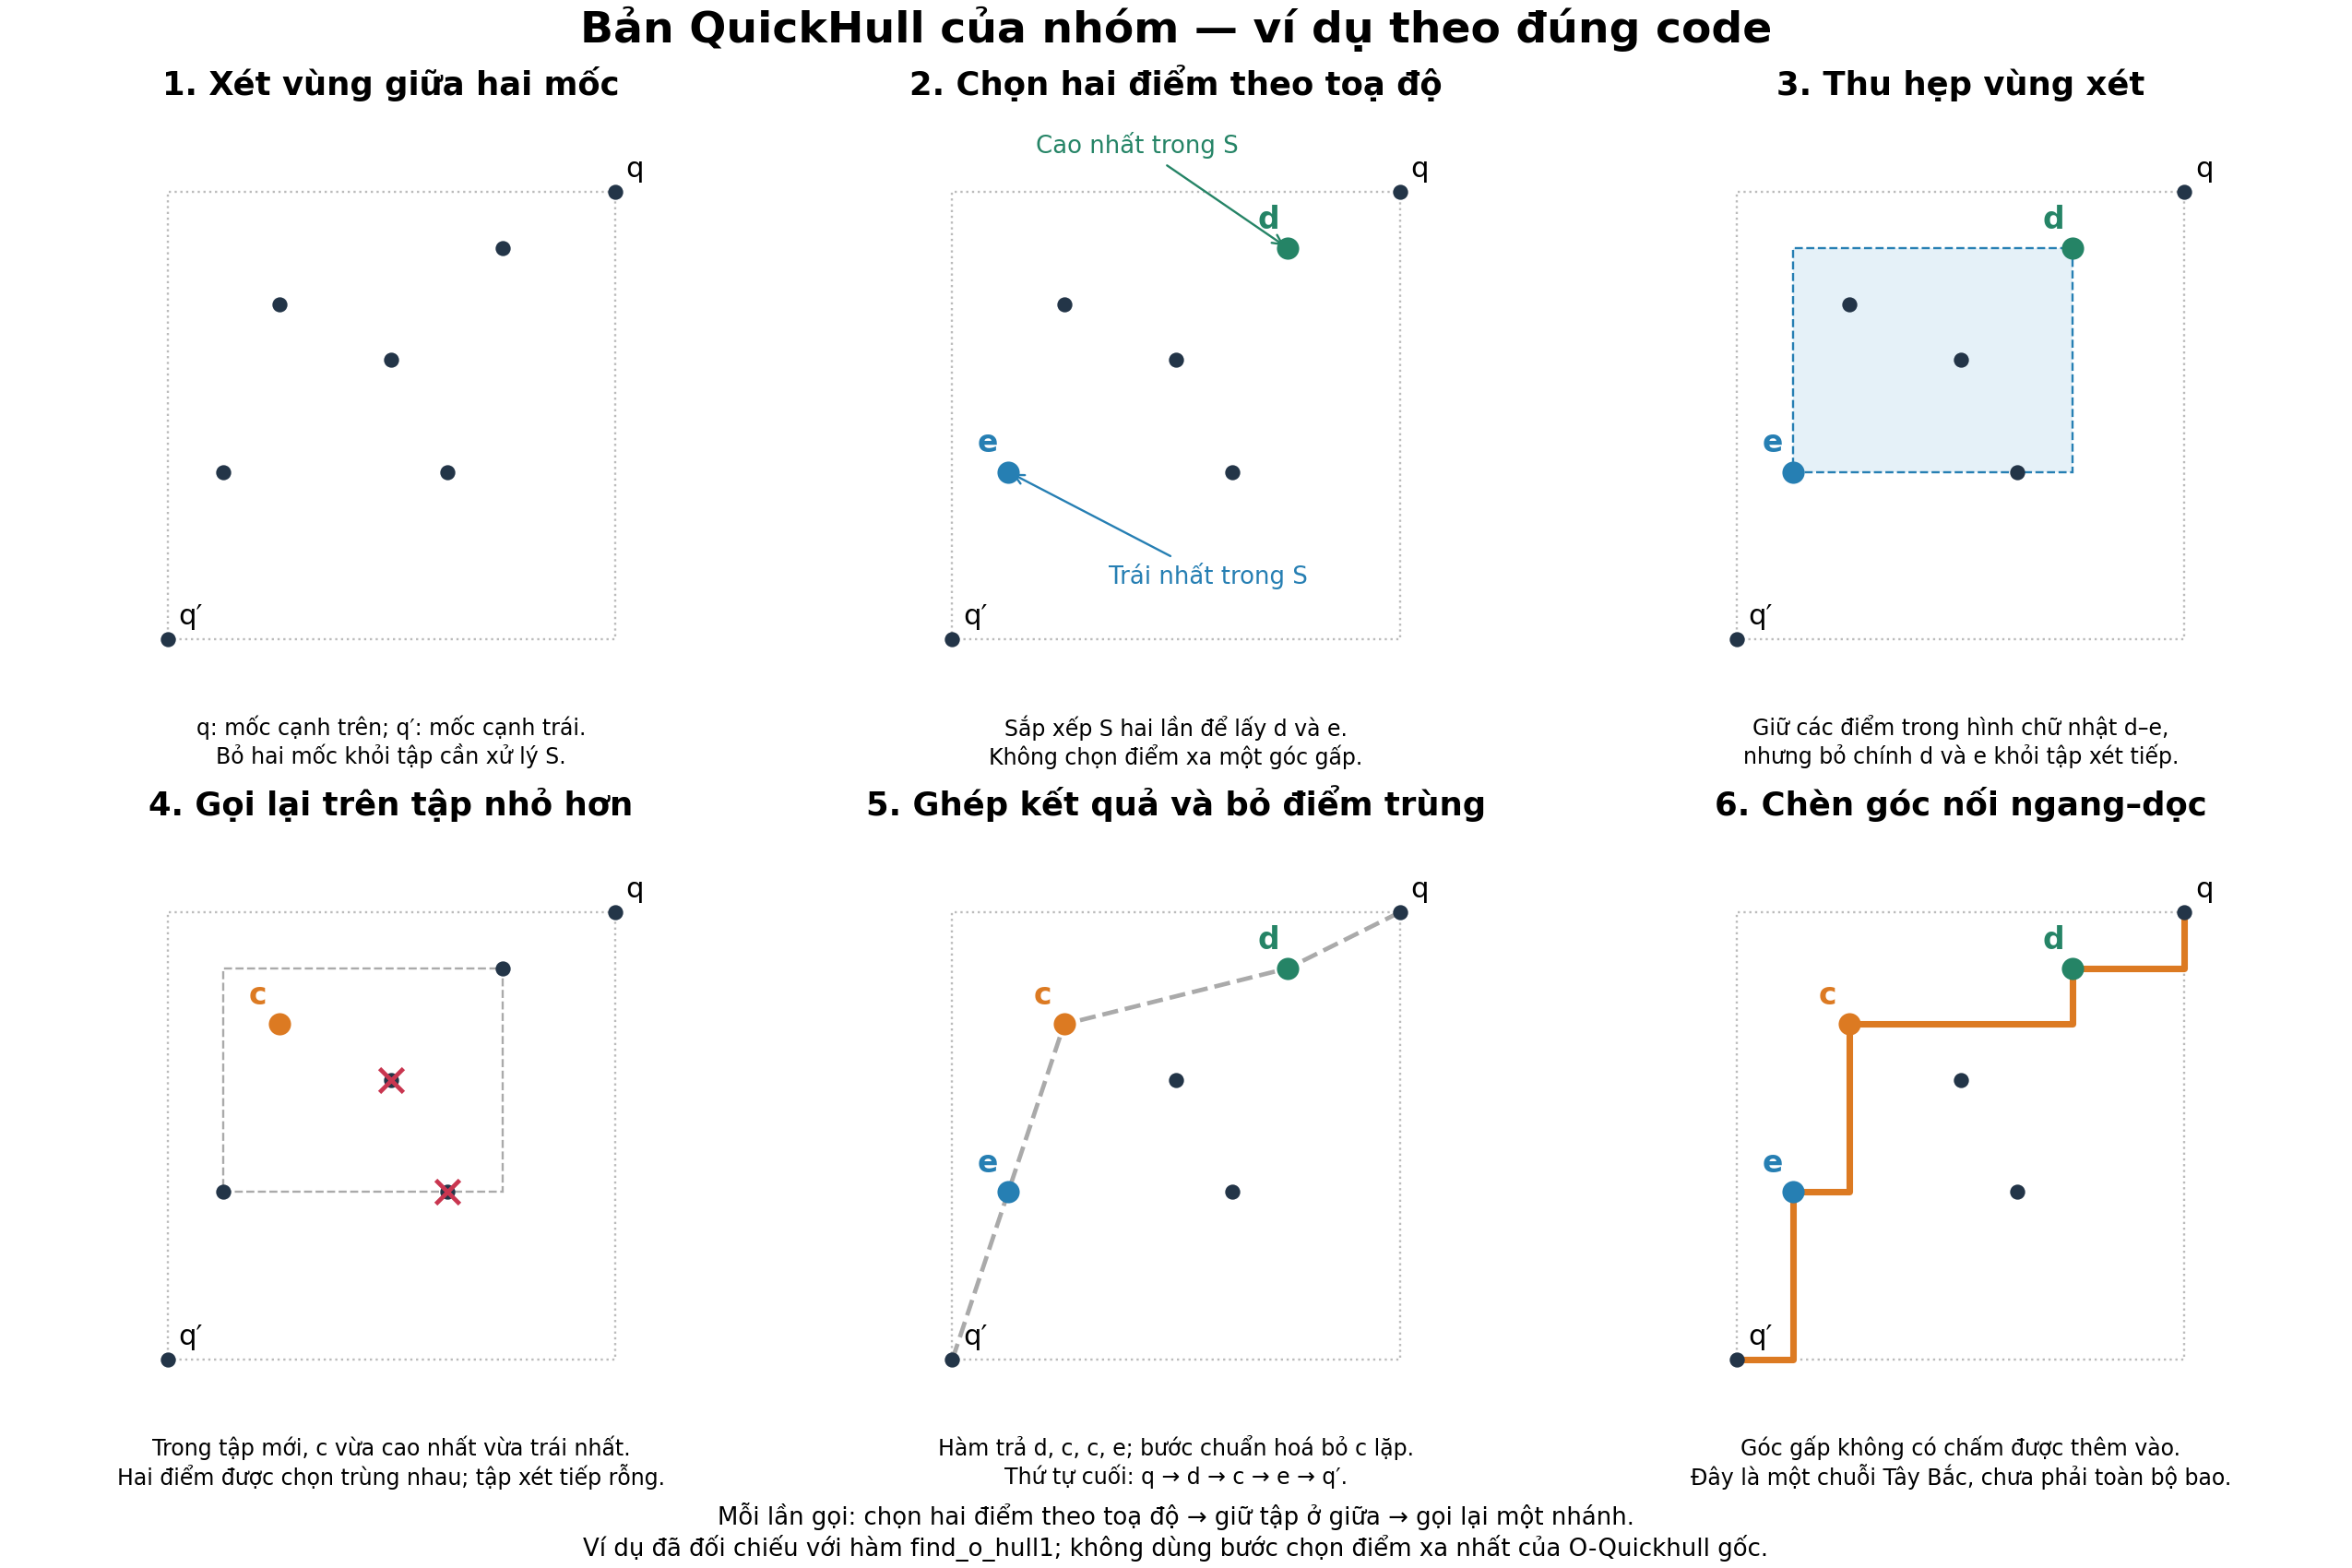
\includegraphics[width=\linewidth]{recursive_group_steps.png}
\caption[Minh hoạ bản QuickHull của nhóm]{Các bước tìm chuỗi Tây Bắc theo bản cài đặt của nhóm. Mã chọn $d$ cao nhất và $e$ trái nhất, rồi xử lý tập nằm giữa chúng để tìm $c$. Sau khi bỏ điểm trùng, các điểm được ghép theo thứ tự $q,d,c,e,q'$ và chèn góc nối. Hình chỉ minh hoạ một chuỗi, chưa phải toàn bộ bao.}
\label{fig:recursive_steps}
\end{figure}

Trong giả mã QuickHull, $A$ là dãy kết quả ghép bốn chuỗi; $S_k$ là tập điểm nằm giữa hai mốc của chuỗi thứ $k$, không gồm hai mốc. Ký hiệu $[]$ là dãy rỗng. Hàm tìm chuỗi của bản QuickHull chỉ trả về các điểm trung gian; phần chính đưa hai mốc vào đầu và cuối. Chỉ số $k=1,2,3,4$ lần lượt ứng với Tây Bắc, Tây Nam, Đông Nam và Đông Bắc. Ký hiệu $\operatorname{Rect}(a,b)$ là hình chữ nhật có hai đỉnh đối diện $a,b$. Ký hiệu $\operatorname{Inside}(S,a,b)$ chỉ các điểm của $S$ nằm trong hoặc trên biên hình chữ nhật này, nhưng không gồm chính $a,b$:
\[
\operatorname{Inside}(S,a,b)=\{p\in S\setminus\{a,b\}:p\in\operatorname{Rect}(a,b)\}.
\]

\begin{algorithm}[H]
\SetAlgoLined
\LinesNumbered
\caption{Bản QuickHull (cài đặt của nhóm)}
\label{alg:quickhull}
\KwIn{Tập điểm $P$, $|P|=n\ge 4$}
\KwOut{Dãy đỉnh của bao lồi trực giao liên thông, theo thứ tự quanh biên}
Tìm $x_{\min},x_{\max},y_{\min},y_{\max}$ và các mốc $q_1,q'_1,\dots,q_4,q'_4$\;
\For{$k\gets 1$ \KwTo $4$}{
  $S_k\gets\operatorname{Inside}(P,q_k,q'_k)$ \tcp*{các điểm giữa hai mốc, không gồm hai mốc}
}
$A\gets []$\;
\For{$k\gets 1$ \KwTo $4$}{
  Nối vào $A$: $q_k$, $\textsc{FindChain}_k(S_k)$, $q'_k$\;
}
Với mỗi cặp đỉnh liên tiếp của $A$ khác nhau ở cả hai toạ độ, chèn một đỉnh góc $90^\circ$\;
\Return $A$\;
\BlankLine
\SetKwFunction{FC}{FindChain$_1$}
\SetKwProg{Fn}{Hàm}{:}{}
\Fn{\FC{$S$}}{
  \If{$S=\emptyset$}{\Return dãy rỗng}
  $a\gets$ điểm cao nhất của $S$ (nếu bằng nhau, lấy điểm bên trái nhất) \tcp*{sắp xếp $S$}
  $b\gets$ điểm trái nhất của $S$ (nếu bằng nhau, lấy điểm cao nhất) \tcp*{sắp xếp $S$}
  \Return $a$, \FC{$\operatorname{Inside}(S,a,b)$}, $b$\;
}
\end{algorithm}

Ba hàm $\textsc{FindChain}_2$, $\textsc{FindChain}_3$, $\textsc{FindChain}_4$ có cùng cách thu hẹp tập điểm, nhưng đổi hướng chọn điểm cho các chuỗi Tây Nam, Đông Nam và Đông Bắc. Độ phức tạp của hai bản cài đặt được tóm tắt trong Bảng~\ref{tab:algo_compare}.

% =====================================================================
\section{Bản Graham của nhóm}
\label{sec:ograham}
\label{sec:impl_ograham}

Thuật toán Graham~\cite{graham1972} tìm bao lồi bằng cách sắp xếp các điểm rồi quét một lượt duy nhất.
Phan Thanh An và cộng sự~\cite{an2021ograham} cải biên ý tưởng này cho bao lồi trực giao liên thông (gọi tắt là \emph{O-Graham}):
thay vì sắp xếp theo góc, các điểm được sắp xếp theo toạ độ; thay vì kiểm tra rẽ trái/rẽ phải,
chỉ cần so sánh một toạ độ để biết điểm có nằm trên chuỗi bậc thang hay không.

Để minh hoạ cách sắp xếp và quét, Thuật toán~\ref{alg:ograham} trình bày bản cài đặt của nhóm theo ý tưởng O-Graham. Đây không phải giả mã sao chép từ bài báo gốc; nhóm chưa đối chiếu từng bước để khẳng định hai bản hoàn toàn tương đương. Trong giả mã, $(s,e)$ là hai mốc đầu--cuối của chuỗi đang xét; $R$ là tập điểm trong hình chữ nhật giữa hai mốc; $C$ là dãy điểm được giữ cho chuỗi đó; $H$ là dãy kết quả ghép bốn chuỗi. Ký hiệu $\operatorname{last}(C)$ là điểm cuối của $C$. Khoá sắp xếp là thứ tự ưu tiên các toạ độ khi xếp điểm, được nêu cho cả bốn hướng ở Bảng~\ref{tab:scan_keys}.

Với chuỗi Tây Bắc, bản Graham của nhóm thực hiện theo các bước sau:
\begin{enumerate}
  \item \textbf{Lấy vùng cần xét.} Giữ các điểm nằm trong hình chữ nhật giữa hai mốc của chuỗi; bắt đầu dãy kết quả bằng mốc trên cạnh trên.
  \item \textbf{Sắp xếp vùng một lần.} Xếp điểm từ cao xuống thấp; các điểm cùng độ cao được xếp từ trái sang phải.
  \item \textbf{Duyệt theo thứ tự đã sắp.} Chỉ thêm một điểm nếu nó nằm bên trái điểm cuối đang giữ. Vì các điểm cùng độ cao đã được xếp từ trái sang phải, chỉ điểm trái nhất của hàng đó có thể được thêm; các điểm còn lại tự không thoả điều kiện đi xa hơn về trái. Nhờ đó, chuỗi tiến dần từ cạnh trên sang cạnh trái.
  \item \textbf{Hoàn thiện chuỗi.} Sau khi duyệt hết vùng, chèn các góc ngang--dọc giữa những điểm nằm chéo nhau. Làm tương tự cho ba hướng còn lại với thứ tự sắp xếp và hướng so sánh tương ứng.
\end{enumerate}

Hình~\ref{fig:ograham_steps} dùng cùng tập điểm với Hình~\ref{fig:recursive_steps}. Hai cách cho cùng chuỗi trong ví dụ, nhưng bản Graham không gọi đệ quy và không sắp xếp lại tập điểm ở từng bước duyệt.

\begin{figure}[H]
\centering
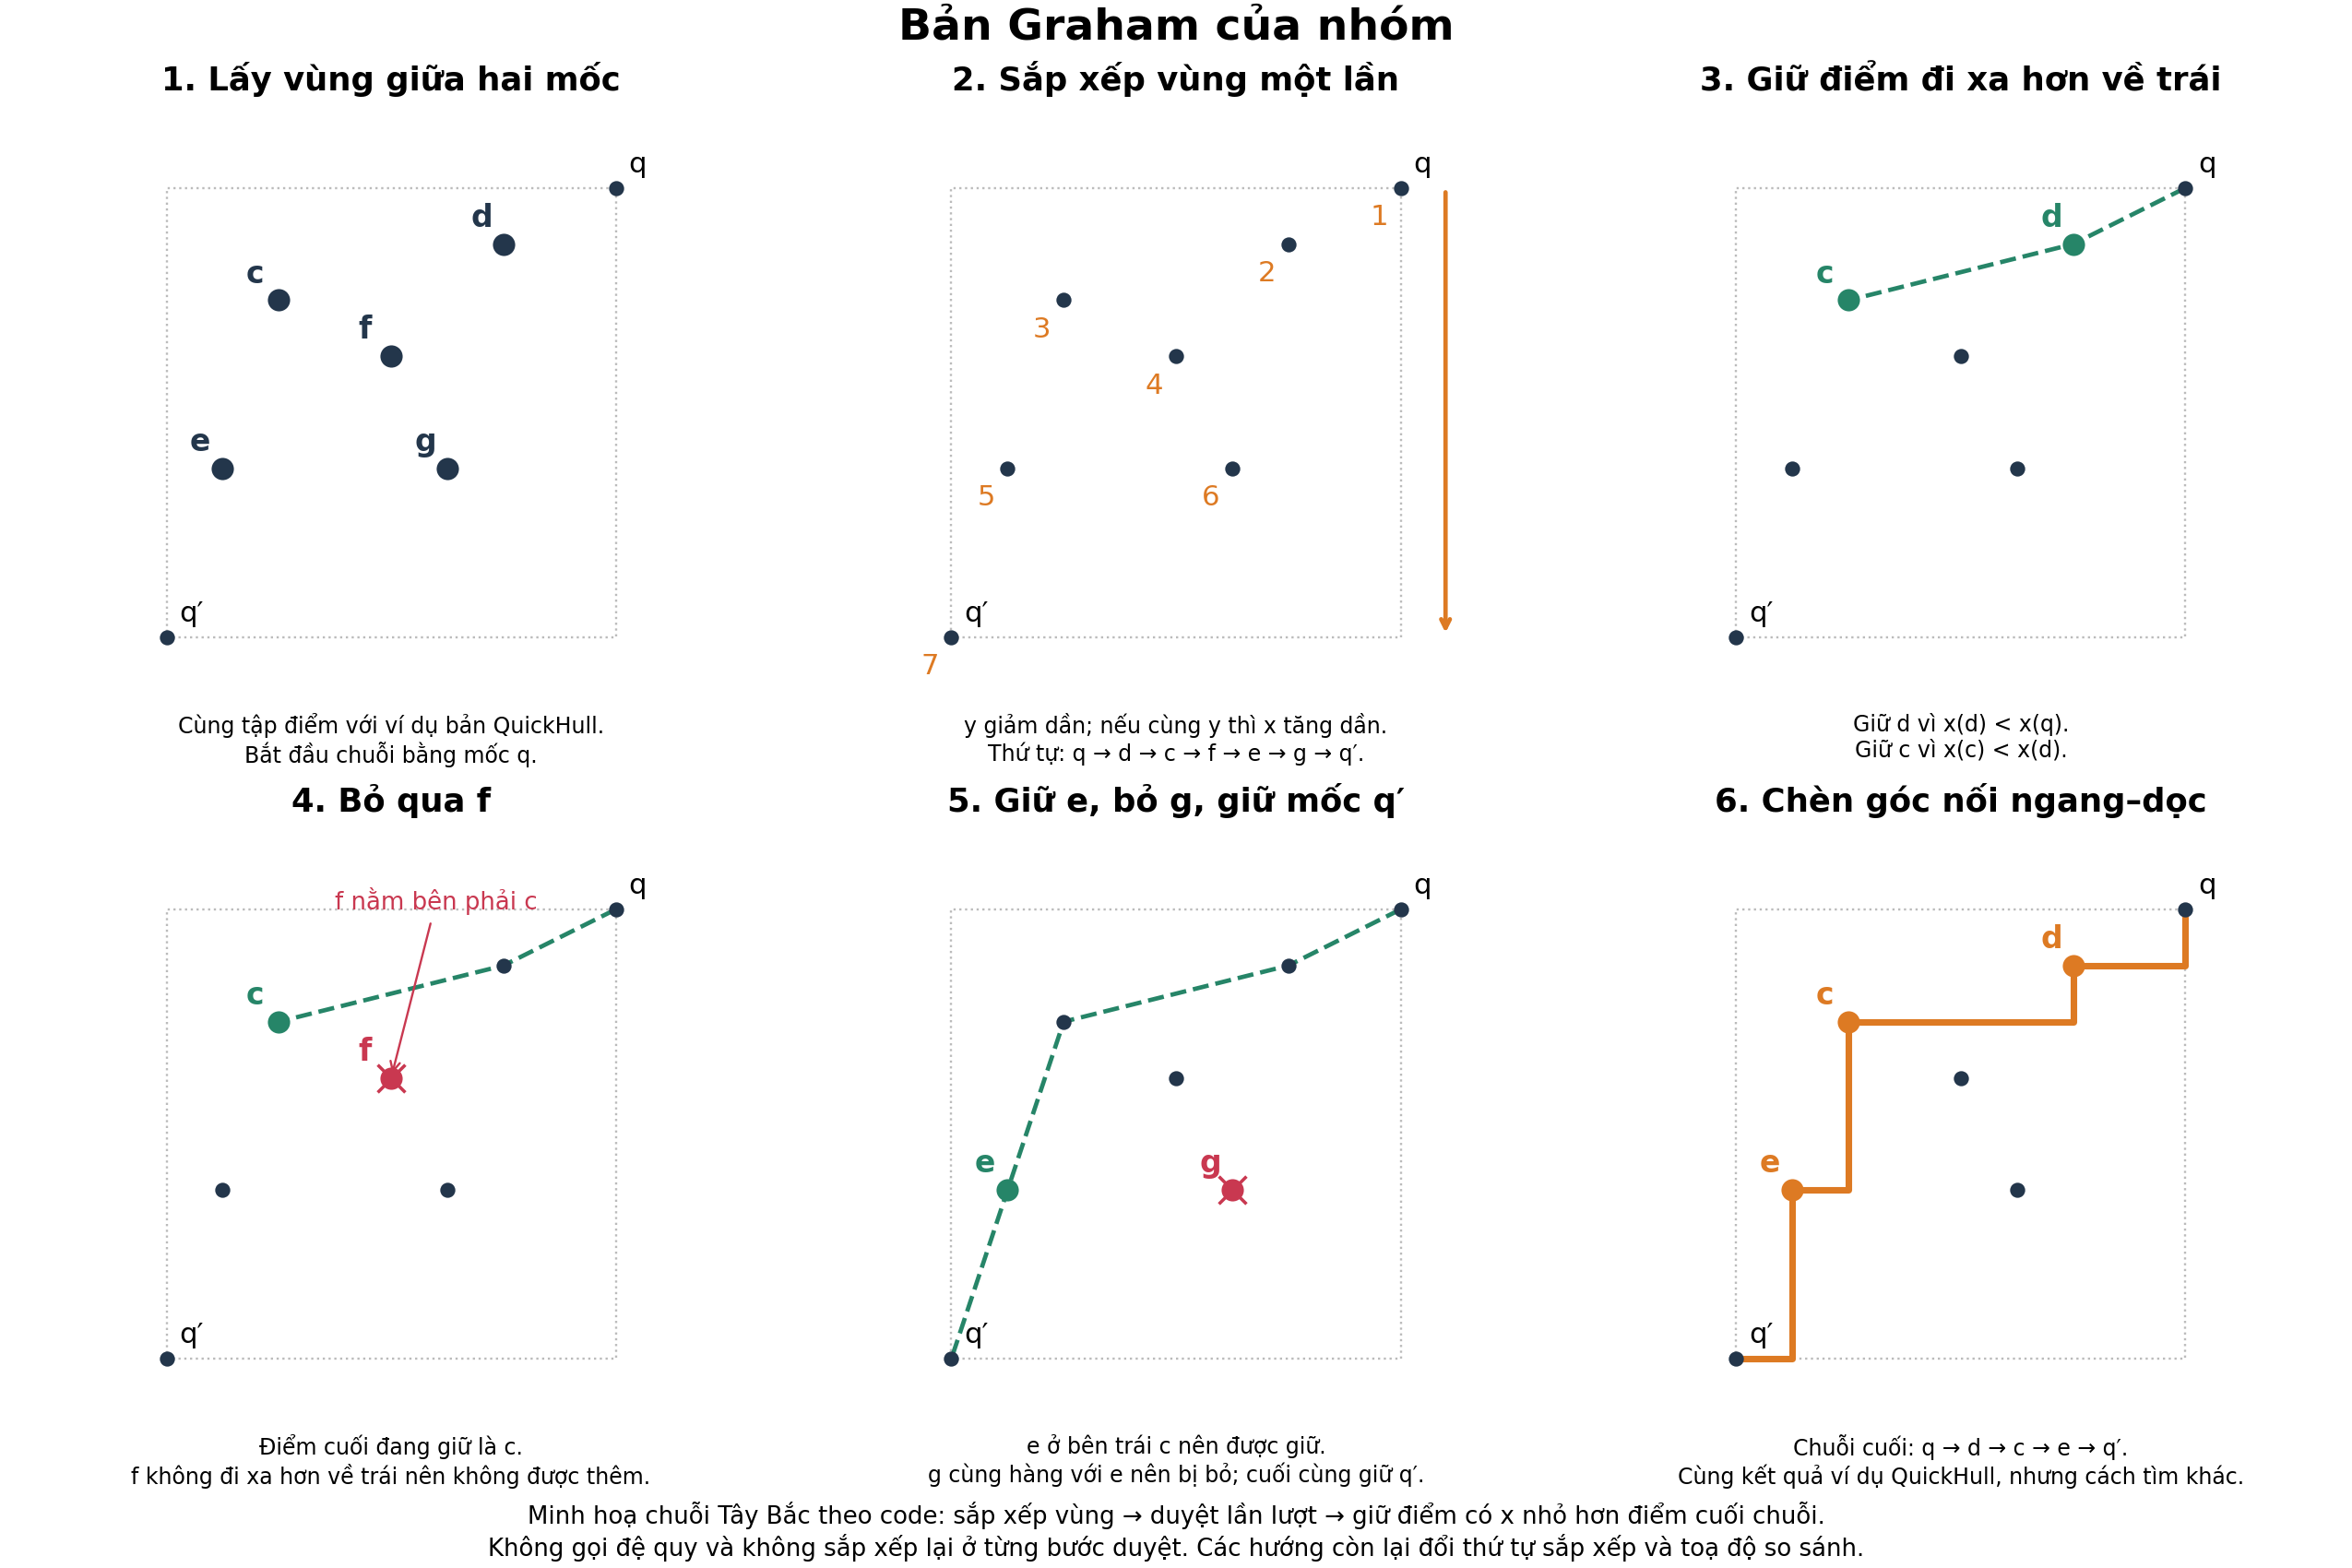
\includegraphics[width=\linewidth]{ograham_group_steps.png}
\caption[Minh hoạ bản Graham]{Các bước tìm chuỗi Tây Bắc theo bản Graham của nhóm. Duyệt từ cao xuống thấp, giữ $d,c,e$ vì chúng lần lượt đi xa hơn về trái; bỏ $f$ vì nằm bên phải $c$ và bỏ $g$ vì không nằm bên trái $e$. Sau khi duyệt và chèn các góc nối, thu được cùng chuỗi như ví dụ bản QuickHull. Hình chỉ minh hoạ một chuỗi biên.}
\label{fig:ograham_steps}
\end{figure}

\begin{algorithm}[H]
\SetAlgoLined
\LinesNumbered
\caption{Bản Graham (cài đặt của nhóm)}
\label{alg:ograham}
\KwIn{Tập điểm $P$, $|P|=n$}
\KwOut{Dãy đỉnh của bao lồi trực giao liên thông, theo thứ tự quanh biên}
Tìm $x_{\min},x_{\max},y_{\min},y_{\max}$ và các điểm mốc\;
$H\gets []$\;
\ForEach{chuỗi $k\in\{\text{Tây Bắc},\text{Tây Nam},\text{Đông Nam},\text{Đông Bắc}\}$}{
  $(s,e)\gets$ điểm mốc đầu và cuối của chuỗi $k$\;
  $R\gets\{p\in P:p\in\operatorname{Rect}(s,e)\}$\;
  Sắp xếp $R$ theo khoá của chuỗi $k$ \tcp*{Tây Bắc: $y$ giảm dần, $x$ tăng dần}
  $C\gets [s]$\;
  \ForEach{$p\in R$ theo thứ tự đã sắp}{
    \If{$p$ vượt điểm cuối của $C$ theo hướng quét của chuỗi $k$}{
      Thêm $p$ vào cuối $C$ \tcp*{Tây Bắc: $p_x<\operatorname{last}(C)_x$}
    }
  }
  Nối dãy $C$ vào cuối $H$\;
}
Với mỗi cặp đỉnh liên tiếp của $H$ khác nhau ở cả hai toạ độ, chèn một đỉnh góc $90^\circ$\;
\Return $H$\;
\end{algorithm}

\begin{table}[H]
\centering
\caption{Khoá sắp xếp và hướng quét của bốn chuỗi}
\label{tab:scan_keys}
\begin{tabular}{lll}
\toprule
Chuỗi & Khoá sắp xếp & Điểm được giữ khi \\
\midrule
Tây Bắc & $y$ giảm dần, rồi $x$ tăng dần & $x$ nhỏ hơn điểm cuối của chuỗi \\
Tây Nam & $x$ tăng dần, rồi $y$ tăng dần & $y$ nhỏ hơn điểm cuối của chuỗi \\
Đông Nam & $y$ tăng dần, rồi $x$ giảm dần & $x$ lớn hơn điểm cuối của chuỗi \\
Đông Bắc & $x$ giảm dần, rồi $y$ giảm dần & $y$ lớn hơn điểm cuối của chuỗi \\
\bottomrule
\end{tabular}
\end{table}


% =====================================================================
\section{Các công trình liên quan}
\label{sec:related}

Phan Thanh An, Phong Thi Thu Huyen và Nguyen Thi Le~\cite{an2021ograham} đề xuất O-Graham để tìm bao lồi trực giao liên thông bằng cách sắp xếp và quét các điểm. Nghiên cứu này là cơ sở tham khảo cho bản Graham của đồ án.

Nguyen Kieu Linh, Phan Thanh An và Tran Van Hoai~\cite{nguyen2022quickhull} đề xuất O-Quickhull, vận dụng ý tưởng chia để trị để tìm các điểm cực trị của bao. Đồ án tham khảo hướng tiếp cận đệ quy này, nhưng bản cài đặt của nhóm chọn điểm theo toạ độ, khác với cách chọn điểm của thuật toán gốc.

Nguyen Kieu Linh~\cite{linh2025parallel} tiếp tục nghiên cứu cách dựng bao hiệu quả cho tập điểm lớn, kết hợp loại bớt điểm không cần xét và xử lý song song. Đồ án chỉ tham khảo hướng phát triển này, chưa cài đặt phương pháp của bài báo.

Từ các nghiên cứu trên, đồ án tập trung ứng dụng bao lồi trực giao để biểu diễn vùng phương tiện. Các phép so sánh tốc độ trong báo cáo chỉ áp dụng cho hai bản cài đặt của nhóm, không phải đánh giá lại hiệu năng của các thuật toán gốc.

% =====================================================================
\section{Theo vết trên video bằng ByteTrack}
\label{sec:tracker}

Theo vết là ghép các phát hiện của cùng một xe qua nhiều khung hình để duy trì một mã định danh (ID). Đồ án sử dụng ByteTrack~\cite{zhang2022bytetrack} có sẵn trong thư viện Ultralytics~\cite{yolo11}, thông qua lệnh \texttt{model.track()} với cấu hình \texttt{bytetrack.yaml}; không tự xây dựng bộ theo vết.

ByteTrack ước lượng vị trí tiếp theo và ghép các hộp dựa trên mức chồng lấp. Các phát hiện có độ tin cậy cao được ghép trước; phát hiện có độ tin cậy thấp vẫn có thể được dùng để nối lại vết đang có. Trong đồ án, tracking chỉ hỗ trợ gắn ID cho phần minh hoạ video, không phải nội dung nghiên cứu chính và không tham gia các phép đánh giá trên ảnh.

% =====================================================================
\section{Độ đo đánh giá}
\label{sec:metrics}

Phần này giải thích các chỉ số dùng trong báo cáo. Các chỉ số đều có giá trị từ 0 đến 1 (hoặc 0\% đến 100\%), càng cao càng tốt.

\paragraph{IoU: hai vùng trùng nhau bao nhiêu.} IoU (Intersection over Union) lấy phần chung của hai vùng chia cho toàn bộ phần chúng phủ.
Với vùng dự đoán $A$ và vùng nhãn chuẩn $B$, tính trên điểm ảnh:
\begin{equation}
  \operatorname{IoU}(A, B) = \frac{|A\cap B|}{|A\cup B|}.
\end{equation}
IoU bằng 1 khi hai vùng trùng khít, bằng 0 khi không chồng lên nhau. Ví dụ, phần chung 80 điểm ảnh và phần phủ 100 điểm ảnh cho IoU bằng 0,8.

\paragraph{Đúng, sai và bỏ sót.} Mỗi dự đoán của mô hình có một \emph{độ tin cậy}, cho biết mô hình chắc chắn đến đâu; dự đoán dưới ngưỡng đã chọn bị bỏ qua.
Một dự đoán được tính là đúng nếu cùng lớp với một nhãn và có IoU với nhãn đó từ 0,5 trở lên; mỗi nhãn chỉ được ghép với một dự đoán, ưu tiên dự đoán có độ tin cậy cao hơn. Trong đánh giá phát hiện đối tượng, báo cáo sử dụng ba loại kết quả TP, FP và FN:
\begin{itemize}
  \item \textbf{TP} (true positive): dự đoán đúng;
  \item \textbf{FP} (false positive): dự đoán sai, tức báo có xe nhưng không ghép được với nhãn nào;
  \item \textbf{FN} (false negative): bỏ sót, tức có nhãn xe nhưng không dự đoán nào ghép được.
\end{itemize}

\paragraph{Precision, Recall và F1.} \emph{Precision} trả lời: trong các xe mô hình báo, bao nhiêu phần là đúng? \emph{Recall} trả lời: trong các xe thật, mô hình tìm được bao nhiêu phần?
Hai chỉ số này thường đánh đổi nhau: báo nhiều hơn thì ít bỏ sót hơn nhưng dễ báo sai hơn. \emph{F1} gộp cả hai thành một số, và chỉ cao khi cả hai cùng cao.
\begin{equation}
  \mathrm{Precision} = \frac{\mathrm{TP}}{\mathrm{TP}+\mathrm{FP}},\qquad
  \mathrm{Recall} = \frac{\mathrm{TP}}{\mathrm{TP}+\mathrm{FN}},\qquad
  F_1 = \frac{2\cdot\mathrm{Precision}\cdot\mathrm{Recall}}{\mathrm{Precision}+\mathrm{Recall}}.
\end{equation}

\paragraph{AP, mAP50 và mAP50--95.} Precision, Recall và F1 phụ thuộc vào một ngưỡng độ tin cậy cố định. \emph{AP} (Average Precision) đánh giá mô hình trên mọi ngưỡng:
nó là diện tích dưới đường cong Precision--Recall của một lớp xe~\cite{everingham2010voc,padilla2021metrics}, nên cao khi mô hình tìm được nhiều xe mà vẫn ít báo sai.
\emph{mAP} (mean AP) là trung bình AP của các lớp xe.
\begin{itemize}
  \item \textbf{mAP50} dùng ngưỡng IoU 0,5: vùng dự đoán chỉ cần khớp vừa phải với nhãn là được tính đúng.
  \item \textbf{mAP50--95} lấy trung bình trên 10 ngưỡng IoU từ 0,50 đến 0,95: ngưỡng càng cao thì vùng càng phải khớp sát, nên chỉ số này khắt khe hơn và phản ánh rõ độ sát của vùng.
\end{itemize}
Đồ án lấy giá trị Precision tại 101 mức Recall cách đều để tính AP theo kiểu COCO~\cite{padilla2021metrics} bằng bộ tính tự viết, không phải công cụ COCOeval chính thức, nên số liệu chỉ dùng để so sánh nội bộ.
